\documentclass[border=8pt]{standalone}
\usepackage{tikz}
\usetikzlibrary{positioning,arrows.meta,calc,decorations.pathreplacing}
\usepackage[scaled=0.95]{helvet}
\renewcommand{\familydefault}{\sfdefault}
\definecolor{ink}{HTML}{1F2328}\definecolor{muted}{HTML}{57606A}
\definecolor{cS}{HTML}{8250DF}  % Stage 1 lead-lag selector
\definecolor{cEL}{HTML}{2A78D6} % Express Links
\definecolor{cFO}{HTML}{EB6834} % Forecast-only
\definecolor{cRA}{HTML}{1BAF7A} % random
\definecolor{fast}{HTML}{2DA44E}\definecolor{mid}{HTML}{D4A72C}\definecolor{slow}{HTML}{CF222E}
\hyphenpenalty=10000
% node positions: two clusters joined by one bridge (hL -- hR)
\def\nodelist{L1/0/0.5,L2/0/-0.5,L3/0.8/1.0,L4/0.8/0,L5/0.8/-1.0,L6/1.6/0.5,L7/1.6/-0.5,hL/2.35/0,hR/3.35/0,R1/4.1/0.5,R2/4.1/-0.5,R3/4.9/1.0,R4/4.9/0,R5/4.9/-1.0,R6/5.7/0.5,R7/5.7/-0.5}
\def\edgelist{L1/L3,L1/L4,L2/L4,L2/L5,L3/L6,L4/L6,L4/L7,L5/L7,L6/hL,L7/hL,hR/R1,hR/R2,R1/R3,R1/R4,R2/R4,R2/R5,R3/R6,R4/R6,R4/R7,R5/R7}
\def\rnsize{2.6mm}
% \road{prefix}{(shift)}{scale}{fill colour}
\newcommand{\road}[4]{%
  \begin{scope}[shift={#2}, scale=#3]
    \foreach \n/\x/\y in \nodelist {\coordinate (#1\n) at (\x,\y);}
    \foreach \a/\b in \edgelist {\draw[ink!45, line width=0.6pt] (#1\a)--(#1\b);}
    \draw[ink!70, line width=1.8pt] (#1hL)--(#1hR);
    \foreach \n/\x/\y in \nodelist {\node[circle, inner sep=0pt, minimum size=\rnsize, draw=ink!75, line width=0.45pt, fill=#4] at (#1\n) {};}
  \end{scope}}
\tikzset{newlink/.style={-{Stealth[length=2.2mm]}, line width=1.4pt, #1},
         arr/.style={-{Stealth[length=2.6mm]}, line width=1pt, draw=ink!65}}

\begin{document}
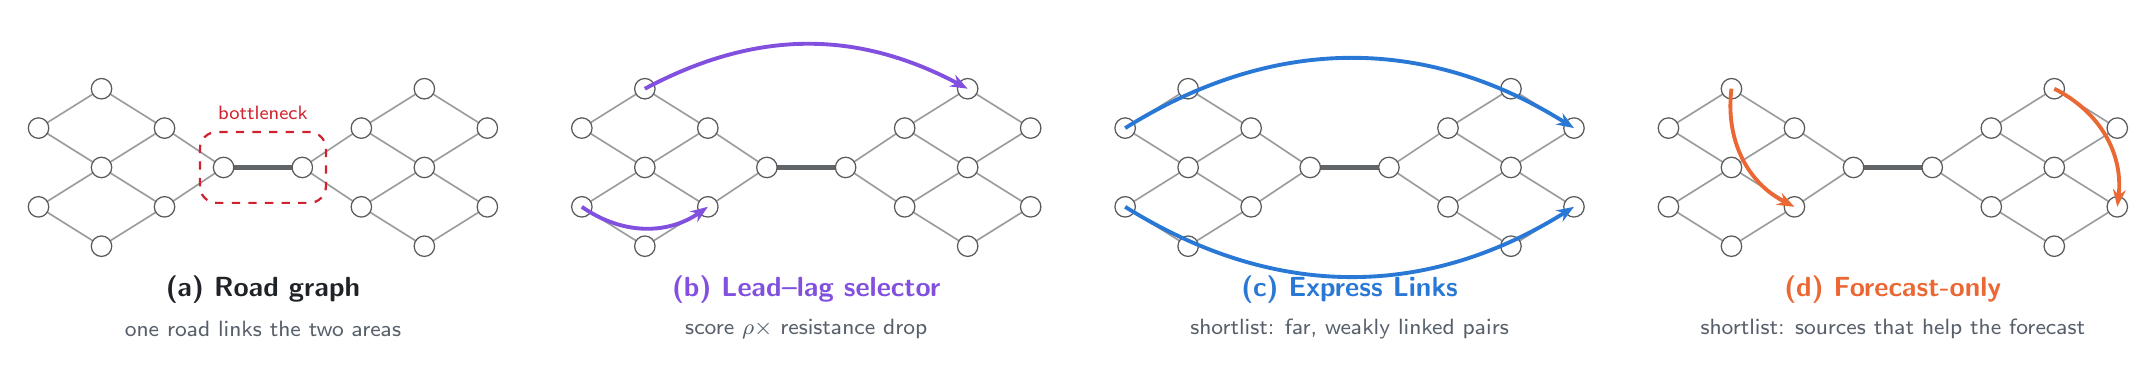
\begin{tikzpicture}[font=\small, color=ink]
\foreach \i/\x in {o/0,s/7.0,e/14.0} {}
% panel helper positions
\def\dx{6.9}
% ---- (a) original
\road{a}{(0,0)}{1}{white}
\draw[slow, dashed, line width=0.8pt, rounded corners=6pt] (2.05,-0.45) rectangle (3.65,0.45);
\node[font=\scriptsize, text=slow] at (2.85,0.7) {bottleneck};
\node[font=\bfseries] at (2.85,-1.55) {(a) Road graph};
\node[font=\footnotesize, text=muted, align=center] at (2.85,-2.05) {one road links the two areas};
% ---- (b) Stage 1 lead-lag selector
\road{b}{(\dx,0)}{1}{white}
\draw[newlink=cS] (bL3) to[bend left=28] (bR3);
\draw[newlink=cS] (bL2) to[bend right=35] (bL7);
\node[font=\bfseries, text=cS] at (\dx+2.85,-1.55) {(b) Lead--lag selector};
\node[font=\footnotesize, text=muted, align=center] at (\dx+2.85,-2.05) {score $\rho\times$ resistance drop};
% ---- (c) Express Links
\road{c}{(2*\dx,0)}{1}{white}
\draw[newlink=cEL] (cL1) to[bend left=32] (cR6);
\draw[newlink=cEL] (cL2) to[bend right=32] (cR7);
\node[font=\bfseries, text=cEL] at (2*\dx+2.85,-1.55) {(c) Express Links};
\node[font=\footnotesize, text=muted, align=center] at (2*\dx+2.85,-2.05) {shortlist: far, weakly linked pairs};
% ---- (d) Forecast-only
\road{d}{(3*\dx,0)}{1}{white}
\draw[newlink=cFO] (dR3) to[bend left=35] (dR7);
\draw[newlink=cFO] (dL3) to[bend right=35] (dL7);
\node[font=\bfseries, text=cFO] at (3*\dx+2.85,-1.55) {(d) Forecast-only};
\node[font=\footnotesize, text=muted, align=center] at (3*\dx+2.85,-2.05) {shortlist: sources that help the forecast};
\end{tikzpicture}
\end{document}
